\chapter{Perspectives}
\label{perspectives}

\begin{quote}
\textit{
In this chapter, we present some research directions emerging from the work presented in this thesis.
A few of these perspectives were already envisioned as long-term objective at the start of our work.
However, other unveiled from our research results and we believe that researching them may yield interesting contributions.
We already started exploring some of these directions.
We first expose how we would like to extend our WebRTC trust and security model in Section~\ref{sec:pemodel}.
Then we propose ways to continue work on the WebRTC IdP Proxy interface in Section~\ref{sec:peproxy}.
Finally, in Section~\ref{sec:pepay} we argue for a comparison of our WebConnect solution with the work of the W3C WebPayment working group.
}
\end{quote}

\glsresetall
\section{On the WebRTC Trust and Security Model}
\label{sec:pemodel}
\subsubsection{Instantiation @Runtime}
We discussed in Section~\ref{sec:webrtcmodelDiscuss} of how we intend to conduct a larger scale survey to validate our trust model.
One of our objective is to integrate the model in to a running WebRTC service to give a sense of context to participants.
Ultimately, the model is to be used by the browser to display a trust and security indicator to the users.
In both situations: the \gls{cs} or the browser running the model, we need to instantiate the model from the actual security configuration, \ie we need to access relevant WebRTC statistics.
We have proposed what we call an \textit{omniscient} view of our WebRTC trust and security model.
To instantiate this omniscient model on an actual WebRTC service, we need to implement a trusted introspection function in the communication setup.
This function would let actors feed their own security information to the model.
The question of trust in these inputs may pose a difficult challenge to solve.

Our contributions focused on ``manual'' reconfiguration of the identity parameters, \ie negotiation and free choice of used \gls{idp} and authentication level.
Our work opened the possibility to work on automatic reconfiguration of a WebRTC session for an increased security level.
It should be our next step in the direction of allowing users to control their WebRTC security.
For instance, we believe that our trust and security model and identity negotiation solution could be integrated with the approach from Alia~\etal\cite{alia2010putting} for dynamic reconfiguration of the security and \gls{qos} parameters.
We believe that setting up this work on a given signalling architecture rather than on a signalling-agnostic approach may help in determining reconfiguration options.
%We did not have time to explore this path and instead focused on ``manual'' reconfiguration, \ie negotiation and free choice of an \gls{idp}.
%One of our initial objective but that we were not able to cover is how to automatically reconfigure the session for more security. 

\subsubsection{Trust Contextualisation}
Another way to contextualise the WebRTC trust and security model could be to explicitly add context information to the trust and security decomposition.
For instance, we considered the possibility to represent explicit context information using a coloured tree in the graphical representation.
Using such formalism means that the decomposition nodes in the model are actually typed.
Firstly, this would allow to express the exact purpose of a trust relation between two actors.
Secondly, the typed decomposition nodes and typed security properties could be extracted from the model.
We believe that researching this direction could open the path of a protocol composition language. 
Such protocol composition language could be used to build on demand security mechanisms based on high-level requirements.

\begin{figure}
\centering
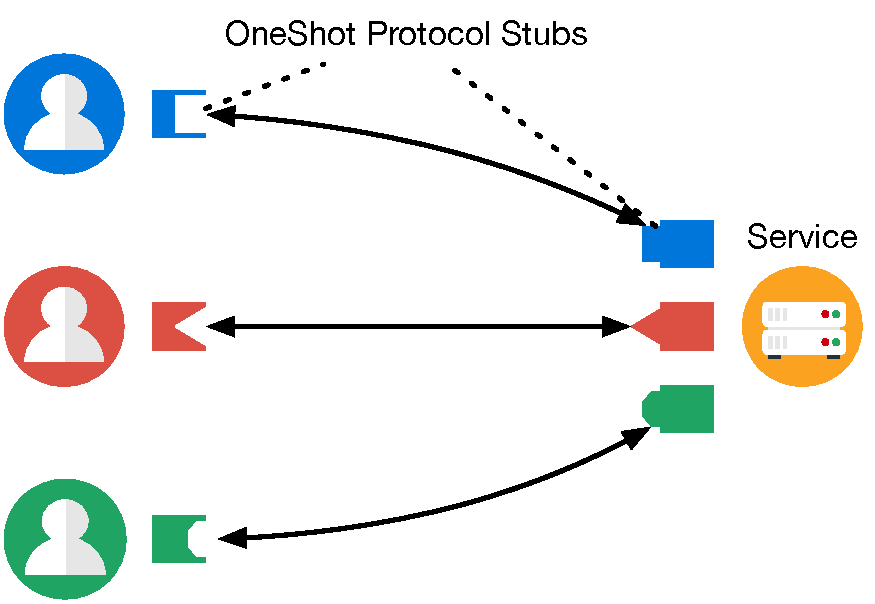
\includegraphics[scale=.5]{images/ossProto}
\caption{One-Shot Protocols Architecture}
\label{fig:oss}
\end{figure}

One possible application of a protocol composition language may be to implement protocol diversification \textit{@Runtime}.
Automatic diversification techniques~\cite{allier15} aim at reducing software mono-culture and its inherent weakness, \ie break-once break-everywhere vulnerabilities.
The idea of automatic protocol diversification is thus to generate protocols on-the-fly for each opened connection.
Whether such architecture would actually increase communication security is an open question.


\section{On the IdP Proxy Interface}
\label{sec:peproxy}
\subsubsection{Loopback Interface}
In some scenarios, especially those for which the WebRTC identity architecture is designed, Alice's \gls{idp} may be the only trusted actor in the communication setup.
Observing our WebRTC trust and security model, we remarked that Alice's \gls{idp} has no influence on Alice's trust in her security.
This is a quite important paradox.
Of course, it is the responsibility of Bob's \gls{idp} to authenticate Bob, but what if this \gls{idp} is also not trusted?
In Section~\ref{sec_sdp}, we proposed a solution to let Alice negotiate which \gls{idp} may be used by Bob.
However, if Alice authenticates too, Alice's \gls{idp} Proxy will be instantiated on Bob's browser.
This is an important asset that could be leveraged so that Alice's \gls{idp} participates in Alice's trust.

Inspired from the ZRTP protocol, a loopback feature, as presented in Figure~\ref{fig:loopback}, could be implemented so that Alice's \gls{idp} confirms who verified the identity assertion.
As Alice's \gls{idp} does not know Bob, this pose some interesting challenges that need to be solved first.
Ultimately, Alice's \gls{idp} may not authenticate Bob on a first call.
Nevertheless, supposing a first secure call, Alice's \gls{idp} may re-authenticate Bob on subsequent call.
A simple solution to implement such mechanism would be to use cookies, as we described in Section~\ref{sec:idptrack}.
Obviously, this implies that the \gls{idp} Proxy interface would have to be modified to incorporate this functionnality.
While the WebRTC identity architecture aims at offering an abstract identity interface, this raise the question as to whether such an interface is possible and how it should be designed.

We would also like the opportunity to explore other mechanisms to authenticate the other peer.
In particular we would like to explore the possibility to fingerprint the other peer's browser through its WebRTC media, stream, and network parameters.
For instance during the \gls{sdp} negotiation, offered and selected \gls{ice} candidates, offered codecs or other parameters may allow to establish a fingerprint of the browser.
It would be interesting to know if such fingerprint could be used in a peer authentication use case or even in a generic web fingerprinting script as in the work of Laperdrix~\etal\cite{laperdrix2016}. 

\begin{figure}[htb]
\centering
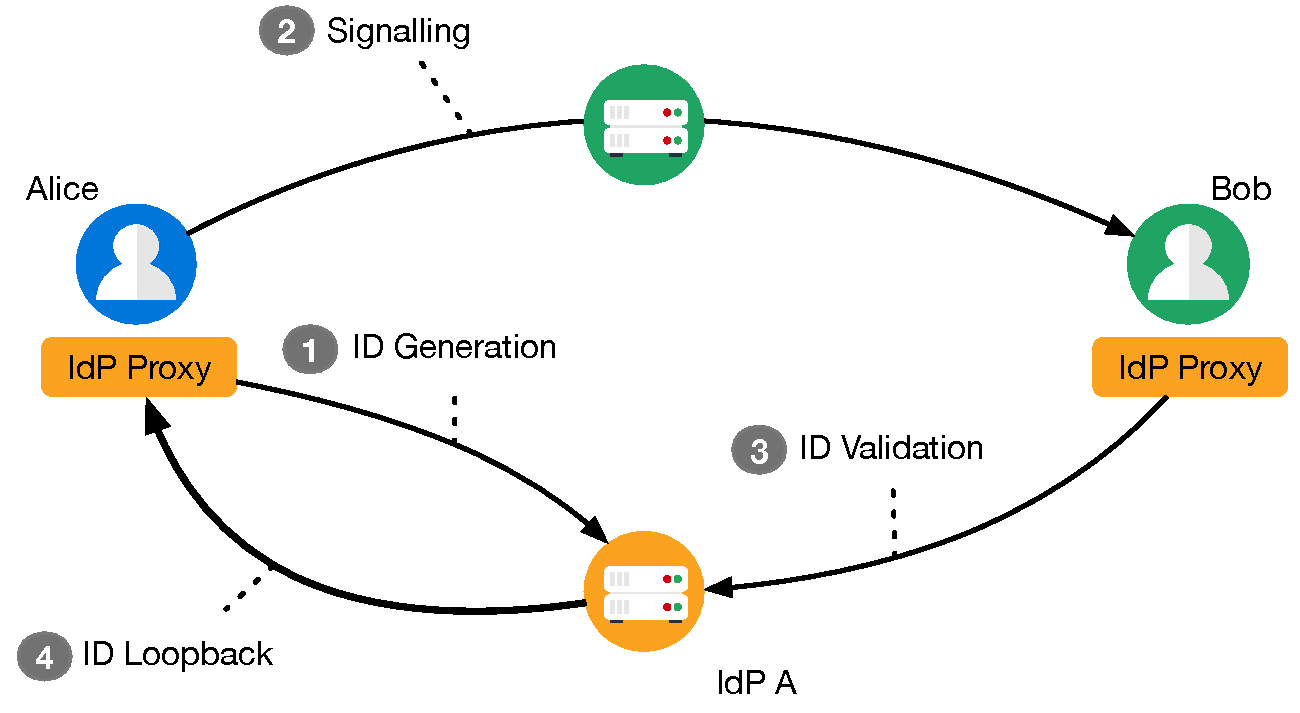
\includegraphics[scale=.5]{images/loopback}
\caption{ID Loopback Sequence}
\label{fig:loopback}
\end{figure}

\subsubsection{WebID TLS Implementation}
WebID~\cite{sporny2011webid} is a distributed identification mechanism which enables each user to control its identity and link to other identities forming a decentralised social network.
A WebID document contains claims of an identity in the resource description framework format and is hosted on a secure domain. 
WebID-TLS~\cite{story2013webid} is an authentication protocol that leverages WebID and \gls{tls} client authentication.
In order to use this protocol, a user first installs its public/private key pair and certificate referring to the WebID document in its browser.
The public key is also added to the user's WebID document.
When a website requires WebID-TLS authentication, the user select its certificate and the browser performs a \gls{tls} client authentication with it.
As the certificate refer to the WebID containing the certificate's public key, the protocol proves to the website that the user is in control of the WebID document, \ie it is authenticated.

Work from the WebID W3C working group seems to have ceased. 
However, as WebID-TLS lets users control their identity and authentication it may be a practical solution to privacy issues related to the role of \gls{idp} on the Web.
We started working on an integration of WebID-TLS with the WebRTC identity architecture during our thesis.
Our idea is to host an \gls{idp} Proxy on the same domain as the WebID, without using any \gls{idp}.
Implementing a WebID-TLS \gls{idp} Proxy would allow users to easily host their identity for WebRTC, for instance on their own blog. 

The main difficulty of this scenario is that the \gls{idp} Proxy must be able to access cryptographic material from the browser stored in client certificates.
For the moment we did not manage to solve this issue and we would like to continue to work on this implementation if given the opportunity.
An alternative solution could be to relax the use of the WebID-TLS protocol and instead rely on WebID-TLS-like approach.
For instance, the \gls{idp} Proxy could use the WebCrypto API~\cite{Watson:17:WCA} to generate, import, and export the private key necessary to sign the identity assertion.
This key could then be stored in the browser storage~\cite{Hickson:16:WSE}.
However, this solution requires to deploy in the WebID host some JavaScript code capable of managing the private key lifecycle, loosing the benefits of the simple WebID-TLS solution.
Ultimately, it may be preferable to integrate the WebCrypto API with the browser exposed interface for \gls{tls} client certificates selection.

\section{On WebConnect and the WebPayment Working Group}
\label{sec:pepay}
In Section~\ref{idpproxyimplem} we have demonstrated that the WebRTC identity architecture can be implemented with OpenID Connect or with a more ad-hoc solution, in Section~\ref{sec_sdp} we have proposed a solution for negotiating the other party identity parameters and in Section~\ref{webconnect} we have adapted the architecture to a user-to-server authentication scenario. 
As we explained in the previous section, we were not able to implement \gls{idp} Proxy with the WebID-TLS protocol and in each other of our solutions we have encountered small issues that restrict some functionalities.
For instance, compared to OpenID Connect, the WebRTC identity architecture does not allow to obtain an authentication strength information or to authenticate the validating party.
In our opinion, \textit{to what extent is the WebRTC identity architecture a generic authentication protocol and what features can be implemented with it} is an interesting and open question.

Web Connect is our solution for letting user choose their identity provider on the Web. 
The work by the \gls{w3c} Web Payment working group recently came to our attention.
This working group proposes a WebPayment \gls{api}~\cite{Denicola:18:PRA} that would let browsers expose an \gls{api} for installing payment application.
Web sites can then use this \gls{api} to request payment to users through the payment application of their choice.
Figure~\ref{fig:webpay} shows a sequence diagram for a payment.
The proposed architecture is actually quite similar to the WebConnect architecture, \ie the payment app is equivalent to the \gls{idp} Proxy, the mediator to the browser, and the payment network to the \gls{idp}.
If the web payment architecture gains traction, it may mean that a similar interface for authentication may benefit from some support. 

\begin{figure}
\centering
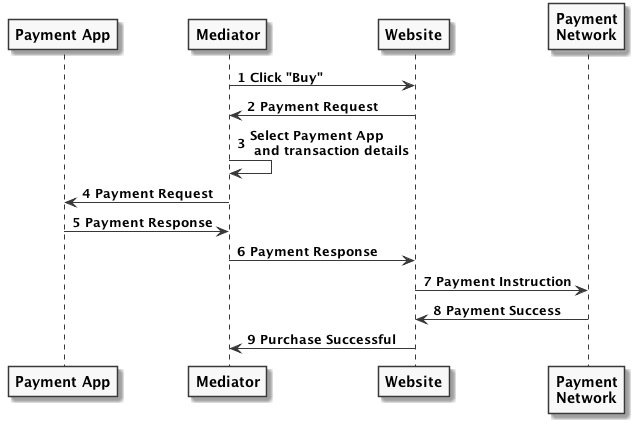
\includegraphics[width=\textwidth]{images/webpayment}
\caption{Payer Makes a Purchase.}
\label{fig:webpay}
\end{figure}


\subsubsection{Offering an Identity Metasystem through the WebPayment API}
In order to promote our solution for freely choosing an \gls{idp}, it may be interesting to explore the similarities between the \gls{idp} Proxy/WebConnect and the WebPayment \gls{api}. 
The parallel between payment and authentication protocol are already known.
For instance the Diameter protocol for authentication, authorization, and accountability can be extended with credit control applications, while spending bitcoins on a blockchain first requires authentication through a private key.
Starting from the idea that emitting a bank cheque with a null value and identity claims is similar to emitting an identity assertion, we would like to test if an authentication protocol can actually be integrated and served through the WebPayment \gls{api}.
This would demonstrate the feasibility of the idea and serve to measure the interest of extending the WebPayment \gls{api} for authentication scenarios.

Going further, the coupling of identity and payment functions in a single API may have additional uses than simply choosing the \gls{idp}.
For instance, some solutions against \gls{spit} propose that users pay an initial fees on first call to deter spammers.
In such solution, if the call is \gls{spit} the money is kept by the callee and the caller is added to a blacklist, if the caller is genuine the money is paid back. 
Supposing that the same interface would offer payment application and peer authentication in WebRTC, such anti-\gls{spit} systems may be quite easy to setup. 

\subsubsection{A generic API for authorization, authentication, and payment}
In this thesis, we have questioned the WebRTC identity architecture as a generic interface for authentication.
We have tested its practical implementation with existing protocols and proposed extensions to other use cases.
In Telco architectures, authentication, authorization, and accounting are regrouped under the term AAA and often provided by the same protocols.
As we remark the similarity between authentication and payment, authentication and authorization are also similar functions as demonstrated by OpenID Connect being an extension to OAuth~2.
We believe that the practicality of a generic interface for all-three AAA functions, for instance considering authentication and accounting as a special case of authentication, may be an interesting research direction.